% begin module piecewise-formula
\begin{frame}
\begin{example}
Find a formula for the function $f$ whose graph is given below.

\psset{xunit=1.2cm, yunit=1.2cm}
\begin{pspicture}(-0.5, -0.5)(5.3,2.4)
\tiny
\psframe*[linecolor=white](-0.5,-0.5)(5.2,2.4)
\psaxes{<->}(0,0)(-0.5,-0.5)(5.2,2.2)
\fcLabels{5.1}{2.2}
\psline[linecolor=red](0,0)(1,1)(2,0)(5,0)
\fcHollowDot{5}{0}
\fcFullDot{0}{0}
\only<handout:0|4-5>{
\psline[linewidth=1.5pt, linecolor=blue](-0.5, -0.5)(2,2)
}
\only<handout:0|6-7>{
\psline[linewidth=1.5pt, linecolor=blue](-0.2, 2.2)(2.5,-0.5)
}
\only<handout:0|8-9>{
\psline[linewidth=1.5pt, linecolor=blue](-0.45, 0)(5,0)
}
\end{pspicture}
%\ \only<1-3,10>{%
%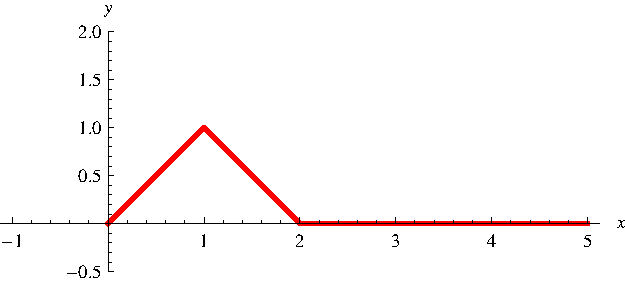
\includegraphics[height=4cm]{precalculus/pictures/01-01-ex-09a.pdf}%
%}%
%\only<handout:0| 4-5>{%
%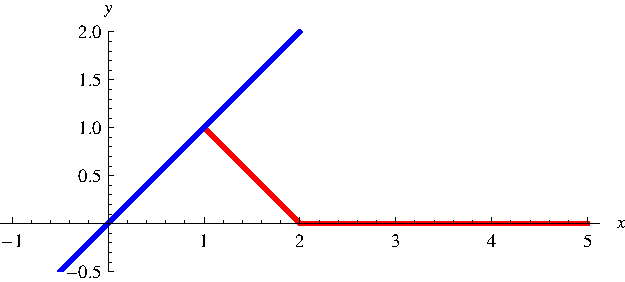
\includegraphics[height=4cm]{precalculus/pictures/01-01-ex-09b.pdf}%
%}%
%\only<handout:0| 6-7>{%
%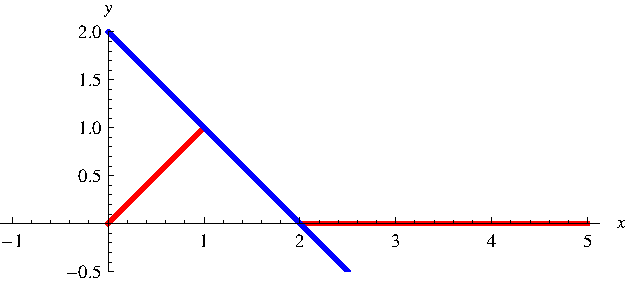
\includegraphics[height=4cm]{precalculus/pictures/01-01-ex-09c.pdf}%
%}%
%\only<handout:0| 8-9>{%
%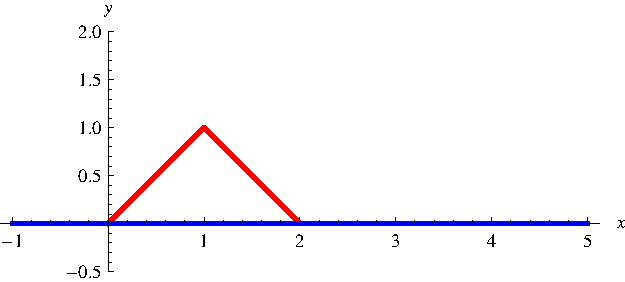
\includegraphics[height=4cm]{precalculus/pictures/01-01-ex-09d.pdf}%
%}%

\uncover<2->{
Different formulas on $[0, 1)$, $[1, 2)$, and $[2, 5)$.
}

\uncover<3->{
\[
\alertNoH{4-9}{f(x) =} \left\{ \begin{array}{ccccccl}
\fcAnswer{5}{x} & \alertNoH{ 4-5}{\text{if}} & \alertNoH{ 4-5}{0} & \alertNoH{ 4-5}{\leq} & \alertNoH{ 4-5}{x} & \alertNoH{ 4-5}{<} & \alertNoH{ 4-5}{1} \\
\fcAnswer{7}{2 - x} & \alertNoH{ 6-7}{\text{if}} & \alertNoH{ 6-7}{1} & \alertNoH{ 6-7}{\leq} & \alertNoH{ 6-7}{x} & \alertNoH{ 6-7}{<} & \alertNoH{ 6-7}{2} \\
\fcAnswer{9}{0} & \alertNoH{ 8-9}{\text{if}} & \alertNoH{ 8-9}{2} & \alertNoH{ 8-9}{\leq} & \alertNoH{ 8-9}{x} & \alertNoH{ 8-9}{<} & \alertNoH{ 8-9}{5} \end{array}\right.
\]
}
\end{example}
\end{frame}
% end module piecewise-formula
